%Simultaneous Localization and Mapping (chpt 07)
\section{Evaluation procedure} \label{evalproc}
To evaluate the performance of the map we create and use a benchmark test.\\
During the evaluation, the drone will first build a map, and then that map will be tested by comparing the real position of the drone with the one it estimates using the map and PnP. The setup used for this evaluation is illustrated on figure \ref{fig:benchmarksetup}.\\
The evaluation is performed as follows:
\begin{enumerate}
  \item The drone is placed in a known position on a table (position A in figure \ref{fig:benchmarksetup}). There, the drone is turned on, and it begins initializing its map by creating a first keyframe.
  \item The drone is then successively placed in 3 other known locations (B, then C, then D), and at each of these locations, the drone manually receives its position. Every time this happens, the drone creates a keyframe, adds landmarks into the map, and optionally updates existing landmarks' positions, or even removes some landmarks.
  \item Finally, the drone is again placed at different known locations (positions 1 through 5 on figure \ref{fig:benchmarksetup}). This time, no information is communicated to the drone from the outside, and the drone does not modify its map. The drone estimates its position using only its camera and the map that it built during step 2. We compare the drone's estimated position with its real position to evaluate the quality of the map.
\end{enumerate}
The two quantities we will seek to optimize are the accuracy of the drone's visual pose estimation (as measured during step 3), and the time taken to create the map during step 2.\\
In reality, the drone would not know its exact position when making keyframes at points B, C, and D (position A is defined as the origin), especially at the beginning, as it would have to rely on its IMU and other internal sensors to estimate its position. To emulate this, we implement a second type of test: the robustness test, where the position that is communicated to the drone is slightly different from its real position, at each of the uncertain points (B, C and D). To differentiate it from the robustness test, we call the first test the precision test.\\
For both the robustness and precision tests, we measure two quantities: the average distance error and average angle error. The average distance error is the average distance in the $xy$-plane between the drone's posistion estimate and its real position when it is at the known points of step 3, and the average angle error is the average absolute value of the difference between the estimated yaw angle and the real yaw angle et these positions. We are not counting errors in roll, pitch, and altitude, because as explained in section \ref{sec:posefusion}, we do not use the result of the visual pose estimate for those quantities, but use the IMU and ultrasound directly. We also do not measure the error when we are moving the drone between those positions, as we do not have the equipment to measure its real position during those transitions.
\begin{figure}[H]
\centering
\begin{subfigure}{\textwidth}
  \centering
  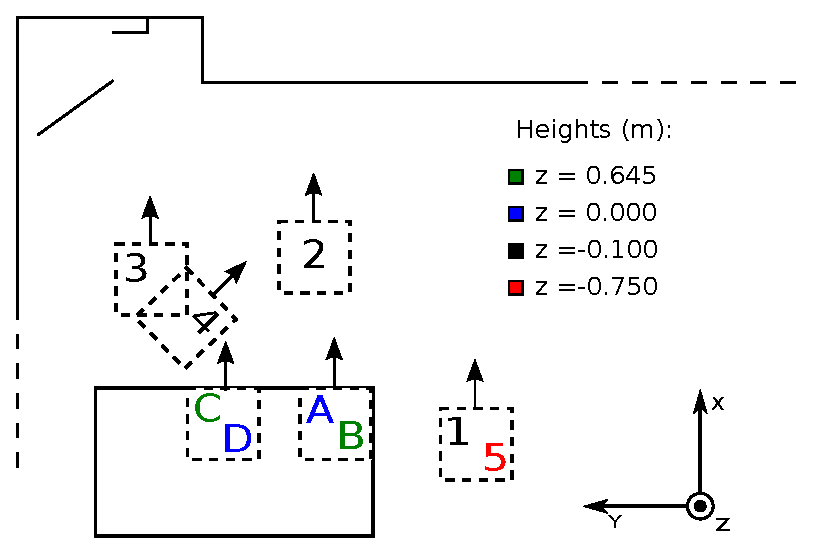
\includegraphics[width=\linewidth]{benchmark_setup.eps}
  \caption{Different positions of the drone during benchmark test}
  \label{fig:benchmarksetup}
\end{subfigure}\\
\vspace{20 mm}
\begin{subfigure}{.33\textwidth}
  \centering
  \includegraphics[width=.99\linewidth]{posA.png}
  \caption{View from position A}
  \label{fig:viewA}
\end{subfigure}%
\begin{subfigure}{.33\textwidth}
  \centering
  \includegraphics[width=.99\linewidth]{posB.png}
  \caption{View from position B}
  \label{fig:viewB}
\end{subfigure}%
\begin{subfigure}{.33\textwidth}
  \centering
  \includegraphics[width=.99\linewidth]{posC.png}
  \caption{View from position C}
  \label{fig:viewC}
\end{subfigure} \\

\begin{subfigure}{.33\textwidth}
  \centering
  \includegraphics[width=.99\linewidth]{posD.png}
  \caption{View from position D}
  \label{fig:viewD}
\end{subfigure}%
\begin{subfigure}{.33\textwidth}
  \centering
  \includegraphics[width=.99\linewidth]{pos1.png}
  \caption{View from position 1}
  \label{fig:view1}
\end{subfigure}%
\begin{subfigure}{.33\textwidth}
  \centering
  \includegraphics[width=.99\linewidth]{pos2.png}
  \caption{View from position 2}
  \label{fig:view2}
\end{subfigure} \\

\begin{subfigure}{.33\textwidth}
  \centering
  \includegraphics[width=.99\linewidth]{pos3.png}
  \caption{View from position 3}
  \label{fig:view3}
\end{subfigure}%
\begin{subfigure}{.33\textwidth}
  \centering
  \includegraphics[width=.99\linewidth]{pos4.png}
  \caption{View from position 4}
  \label{fig:view4}
\end{subfigure}%
\begin{subfigure}{.33\textwidth}
  \centering
  \includegraphics[width=.99\linewidth]{pos5.png}
  \caption{View from position 5}
  \label{fig:view5}
\end{subfigure}

\caption{Views during benchmark test}
\label{fig:benchmarkviews}
\end{figure}

\subsection{Comparison of triangulation methods} \label{sec:comparetriang}
Using the evaluation procedure described in section \ref{evalproc}, we can compare midpoint triangulation and optimal correction. A comparison of their performances can be seen on table \ref{fig:triangcompare}.

\begin{table}[H]
  \centering
  \caption{Comparison between triangulation methods}
  \small\addtolength{\tabcolsep}{-2pt}
  \sisetup{round-mode=places, round-precision = 3}
  \begin{tabular}{ @{} l S[table-format=2.2,round-precision=2] S[table-format=2.1,round-precision=1]
                         S[table-format=2.2,round-precision=2] S[table-format=2.1,round-precision=1] @{}  }
    \toprule
    {}                 & \multicolumn{2}{c}{Accuracy} &  \multicolumn{2}{c}{Robustness} \\
    {}                 & {\footnotesize Distance (\si{\meter})} & {\footnotesize Angle}
                       & {\footnotesize Distance (\si{\meter})} & {\footnotesize Angle} \\
    \midrule
    %Midpoint Method    & \num{0.121729436669}  & \num{0.052339119893} & \num{0.844616151792} & \num{0.27019708855} \\ % radian
    %Optimal Correction & \num{0.0988557438948} & \num{0.0406436455673}& \num{0.775954169079} & \num{0.218538344815}\\ % radian
    Midpoint Method    & \num{0.121729436669}  & \SI{2.9988106732981}{\degree} & \num{0.844616151792} & \SI{15.48115281064}{\degree}\\
    Optimal Correction & \num{0.0988557438948} & \SI{2.3287093550318}{\degree} & \num{0.775954169079} & \SI{12.52132481967}{\degree}\\
      \bottomrule
  \end{tabular}
  \label{fig:triangcompare}
\end{table}

%optimal correc: 24ms
%midpoint      : 12ms

%TODO: put number of matches
We can see that the optimal correction method performs somewhat better. However, this comes at the cost of computation time, because it takes approximately \SI{12}{\milli\second} to triangulate all \num{165} matches between two views using the midpoint method, and \SI{24}{\milli\second} to do the same with the optimal corrction method. In both cases however, this time is insignificant when compared to bundle adjustment (which is performed just after triangulation). For this reason, and the fact that optimal correction is better motivated theoretically and that is gives slightly better results on the benchmark test, we will use optimal correction.\\
It is interesting to see, however, that the difference in performance is much greater between the accuracy and robustness tests than between the two triangulation method. This can be explained by the fact that optimal correction is well suited to correct measurement errors by the camera that follow a normal distribution, but not errors stemming from the fact that the position estimate of the cameras is wrong. That is the reason we need bundle adjustment.

\subsection{Bundle Adjustment}
\begin{table}[H]
  \centering
  \caption{Performance of Bundle Adjustment}
  \small\addtolength{\tabcolsep}{-2pt}
  \sisetup{round-mode=places, round-precision = 3}
  \begin{tabular}{ @{} l S[table-format=2.2,round-precision=2] S[table-format=2.1,round-precision=1] S[table-format=2.3,round-precision=3]
                         S[table-format=2.2,round-precision=2] S[table-format=2.1,round-precision=1] S[table-format=2.3,round-precision=3] @{}  }

    \toprule
    {}      & \multicolumn{3}{c}{Accuracy} &  \multicolumn{3}{c}{Robustness} \\
    {}      & {\scriptsize Distance (\si{\meter})} & {\scriptsize Angle} & {\scriptsize Time (\si{\second})}
            & {\scriptsize Distance (\si{\meter})} & {\scriptsize Angle} & {\scriptsize Time (\si{\second})} \\
    \midrule
    No B.A.  &\num{0.0988557438948}&\SI{2.3287093550318}{\degree}&{\textemdash}&\num{0.775954169079}&\SI{12.52132481967}{\degree}&{\textemdash}\\
    With B.A.&\num{0.0282887755044}&\SI{0.617492395502}{\degree}&\num{0.699653536081}
             &\num{0.0264297442542}&\SI{0.523342243368}{\degree}&\num{2.07235994935}  \\
    \bottomrule
  \end{tabular}
  \label{fig:bacompare}
\end{table}

We see that in the accuracy test, bundle adjustment gives a significant improvement to the performance of the pose estimation. In the robustness test, however, bundle adjustment makes the results quite worse. This is surprising, as it is just in the case where the pose of the camera is uncertain that bundle adjustment should improve the result, by adjusting the pose of the camera. But because the problem is quite non linear, it is possible to fall in local minima. We will later see that by tuning the bundle adjustment phase, we can make it perform much better, and actually improve the results in the robustness test. The other big problem of bundle adjustment is the time it takes. In both tests, this time was over \SI{13}{\second}, which is a prohibitively large amount of time for real time applications. In addition to improving the performance on the robustness test, we will try to reduce the time taken by the bundle adjustment.


\subsection{Tuning the Bundle Adjustment}
The main drawback of Bundle Adjustment is that it requires an iterative method to be solved and can take a lot of time, which of course is a limiting factor for a robot that builds a map in real time. Therefore it is important to optimize both the speed of the computations, and their accuracy. As is often the case, there will have to be a tradeoff between these two goals. To measure both the speed of the Bundle Adjustment and the accuracy of the map obtained, we will conduct some experiments using different parameters to initialize the map.

\subsubsection{Convergence of the solver}
The first element we can tune is the convergence criterion of the solver that solves the bundle adjustment problem. We will stop when the ratio of the change in the objective function to the value of this function arrives below some threshold. This ensures that the criterion scales with the problem, which is important as the size of the problem can vary during operation (as the map grows, for example). The default value of the Ceres solver is $10^{-6}$, but experimentally, we find that we can use a softer threshold to significantly speed up the computations, without impacting the quality of the results too much (and even improving them in the robustness test).

\begin{table}[H]
  \centering
  \caption{Effect of convergence criterion on Bundle Adjustment speed and performance}
  \small\addtolength{\tabcolsep}{-2pt}
  \sisetup{round-mode=places, round-precision = 3}
  \begin{tabular}{ @{} S[scientific-notation=true] S[table-format=1.3] S[table-format=1.3] S[table-format=2.3]
                                                   S[table-format=1.3] S[table-format=1.3] S[table-format=2.3] @{}  }
    \toprule
    \multirow{2}{4em}{Convergence Threshold}  & \multicolumn{3}{c}{Accuracy} &  \multicolumn{3}{c}{Robustness} \\
        & {\scriptsize Distance (\si{\meter})} & {\scriptsize Angle (\si{\radian})} & {\scriptsize Time (\si{\second})}
        & {\scriptsize Distance (\si{\meter})} & {\scriptsize Angle (\si{\radian})} & {\scriptsize Time (\si{\second})} \\
    \midrule
    \num{10}       &\num{0.0988557438948}&\num{0.0406436455673}&\num{0.528740555048}&\num{0.775553503184}&\num{0.219380944042} &\num{0.527468636632} \\
    \num{5}        &\num{0.0988557438948}&\num{0.0406436455673}&\num{0.532568186522}&\num{0.775954169079}&\num{0.218538344815} &\num{0.560289662331} \\
    \num{1}        &\num{0.0988557438948}&\num{0.0406436455673}&\num{0.536680459976}&\num{0.775954169079}&\num{0.218538344815} &\num{0.529257409275} \\
    \num{0.5}      &\num{0.0988557438948}&\num{0.0406436455673}&\num{0.532132491469}&\num{0.284057820455}&\num{0.0860006110714}&\num{0.61461224407}  \\
    \num{0.1}      &\num{0.116334787731} &\num{0.0370860746263}&\num{0.67120449245} &\num{0.244478011775}&\num{0.0982536795903}&\num{1.17620864138}  \\
    \num{0.05}     &\num{0.0684117396072}&\num{0.01622317801}  &\num{0.742543946952}&\num{0.291411483818}&\num{0.112600996782} &\num{2.11719946936}  \\
    \num{0.01}     &\num{0.0895791917611}&\num{0.032296133528} &\num{1.42051474378} &\num{0.823415005012}&\num{0.316300896325} &\num{2.77009601146}  \\
    \num{0.005}    &\num{0.0908954991063}&\num{0.0308365172421}&\num{1.53279625252} &\num{0.142093947791}&\num{0.0495629729962}&\num{4.18590991944}  \\
    \num{0.001}    &\num{0.0849543195902}&\num{0.023134969351} &\num{3.61956872419} &\num{1.034983532}   &\num{0.397193935917} &\num{4.90690393746}  \\
    \num{0.0001}   &\num{0.0842253035954}&\num{0.0258716997751}&\num{5.05812323838} &\num{1.36150222356} &\num{0.479872553731} &\num{10.4840388894}  \\
    \num{0.00001}  &\num{0.0899028376206}&\num{0.0299204957695}&\num{12.4531462789} &\num{1.4834446381}  &\num{0.528430316164} &\num{13.2059885859}  \\
    \num{0.000001} &\num{0.0897626230568}&\num{0.029930165598} &\num{15.7027562261} &\num{1.37414105299} &\num{0.492183127143} &\num{13.8024009466}  \\
    \num{0.0000001}&\num{0.0875171189566}&\num{0.0282118025117}&\num{15.7951563597} &\num{1.55886341652} &\num{0.567309620599} &\num{12.934817493}   \\
    \bottomrule
  \end{tabular}
  \label{tab:convergencetol}
\end{table}

As we can observe on table \ref{tab:convergencetol}, the more severe the convergence threshold, the better the performance on the accuracy test. On the robustness test, however, this is true for high convergence thresholds, but when the convergence threshold is lower than \num{0.01}, the performance starts to degrade as the convergence threshold becomes lower. In both the accuracy and robustness tests, the lower the threshold, the longer it takes. We will chose a threshold of \num{0.05}, as it is a nice compromise of performance on the accuracy test, performance on the robustness test, and speed.
